\chapter{Форматы данных для организации взаимодействия различных программно-аппаратных архитектур}\label{ch:ch3}

\section{Модель размещения данных.}\label{sec:ch3/sect1}

Для описания информации об эволюции численной модели была предложена базовая структура, хранящие данные о состоянии частицы как физические величины: позиция, скорость, ускорение, плотность, масса, вязкость, давление в каждый момент времени так и характеристические такие как идентификатор (\(particleID\)), идентификатор пространственной ячейки (\(cellID\)), тип частицы рисунок ~\ref{fig:p_struct}.
\begin{figure}[ht]
  \centerfloat{
    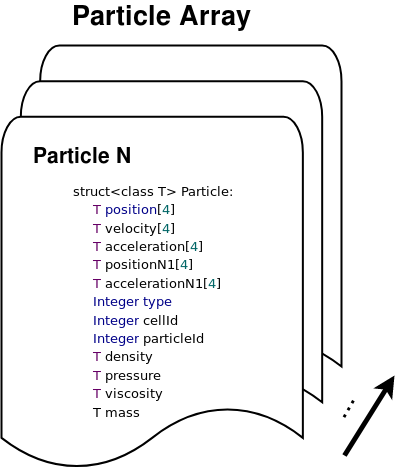
\includegraphics[scale=0.50]{p_struct}
  }
  \caption{Структура частицы.}\label{fig:p_struct}
\end{figure}

Таким образом модель описывается массивом частиц. При этом в зависимости от требования порядку точности вычислений можно варьировать обобщенный тип T между двумя интегральными типами данных \(float\) или \(double\). Каждая партиция определяется следующим образом пусть \(N\) – количество частиц \((p_0,...,p_{N-1})\) – упорядоченное по \(cellID\) множество начальных данных о частицах. Подразумевается, что каждый элемент \(p_i\) хранит пространственные координаты, координаты вектора скорости и \(cellID\) \(i\)-й частицы как показано на рисунке ~\ref{fig:p_struct}. Определим пространственные параметры модели
\((x_{min}, y_{min}, z_{min})\), \((x_{max}, y_{max}, z_{max})\) – точки, определяющие границы области моделирования (вершины параллелепипеда, лежащие на его диагонали).
\(gridCellX\), \(gridCellY\), \(gridCellZ\)- количество пространственных ячеек по соответствующим измерениям трехмерного пространства. Эти значения получаются из целочисленного деления длины ребра ограничивающего объема на длину ребра пространсвенной ячейки например
\[
  gridCellX = \left \lfloor \frac{\left |x_{max} - x_{min}  \right |}{2h} \right \rfloor
\]
\[
  gridCellY = \left \lfloor \frac{\left |y_{max} - y_{min}  \right |}{2h} \right \rfloor
\]
\[
  gridCellZ = \left \lfloor \frac{\left |z_{max} - z_{min}  \right |}{2h} \right \rfloor
\]
\(h\) – радиус сглаживания,
\(M\)– количество доступных устройств.

Для сравнительной оценки производительности устройства вводится эвристическая функция, которая рассчитывает коэффициент производительности на основе возможного количества потоков, которые можно одновременно запустить на конкретном устройстве:
\[
  \epsilon(d_i)=D \cdot WG
\]
где \(d_i\) – устройство, \(D\)- количество доступных стриминговых мультипроцессоров (streaming multiprocessor - SM), для CPU – это число равно количеству ядер, \(WG\) – размерность рабочей группы для конкретного устройства. Например GPU Radeon R 290X обладает 44 стриминговых ядер, \(WG=256\).

Для достижения синхронности времени работы, необходимо, чтобы перед каждой итерацией данные были распределены между устройствами в количестве пропорциональном производительности устройств. Оптимальное количество частиц для обработки \(i\)-ым устройством определяется по следующей формуле:
\[
  N_{i}^{'}=\left [ N \cdot \frac{\epsilon(d_i)}{\sum_{j}\epsilon(d_j)} \right ]
\]

Сформулируем еще два условия:
\noindent
\begin{enumerate}
  \item Все частицы, лежащие одной ячейке, должны обрабатываться одним устройством. Это условие можно сформулировать следующим образом:
        \((C)\) \(\forall p_i, p_j\) \textit{если \(cellID\) частицы \(p_i=cellID\) частицы \(p_i\), то \(p_i, p_j\) обрабатываются одним устройством.}
  \item Количество пространственных ячеек обрабатываемых одним устройством должно быть кратным \(gridCellY\).
\end{enumerate}

Следствием наложения этого условий является то, что итоговое количество частиц \(N_i \) для обработки \(i\)-м устройством  может отличаться от \(N_{i}^{'}\) (в зависимости от количества частиц в ячейке) т.е.:
\[
  N_i = N_{i}^{'}+\Delta N_i, i=0,..., M-1
\]
При этом:
\[
  \sum_{j} N_j = \sum_{j}N_{j}^{'}=N
\]

Введем определение структуры партиции \(partition_i\) – структура для хранения индексов в общем массиве данных первой \(partition_{i}.start\) и следующей после последней частицы \(partition_{i}.end\), обрабатываемой \(i\)-м sudo snap install --classic goустройством с соблюдением условия
\((C)\), которое достигается за счет упорядоченности множества частиц по номеру ячейки.
\[
  partition_{0}.start = 0
\]
\[
  partition_{0}.end = partition_{0}.start + \epsilon (d_0) \cdot N + OFFSET_0
\]
\[
  ...
\]
\[
  partition_{i}.start = partition_{i-1}.end + 1
\]
\[
  partition_{i}.end = partition_{i}.start + \epsilon (d_i) \cdot N + OFFSET_i, i=2,..., M - 1
\]
\(OFFSET_i\) – определяет количество частиц, которые находятся в добавочных ячейках (см. условие 2).
Заданные выше партиции определяют подмножества частиц, обрабатываемые соответствующими устройствами. Таким образом достигается распределение данных между устройствами так, что группы данных не пересекаются друг с другом. Как было уже сказано выше для корректности расчетов для частиц, которые находиться на границах партиций необходимо также учитывать частицы находящиеся в граничных ячейках соседних партиций.Устройство с номером  получает на обработку упорядоченный по  набор частиц. \fixme{К этому набору применяется параллельный метод PCI SPH. // тут нужно дописать}

\section{Алгоритм параллельной сортировки массивов структурированных данных.}\label{sec:ch3/sect2}

Как показывают графики зависимости производительности от количества частиц для различных конфигураций время вычисления одной итерации моделирования сильно коррелирует с процессом синхронизации и, в значительной мере, сортировке ~\ref{fig:result}. Для  конфигураций с количеством частиц, начиная от нескольких миллионов, сортировка может занимать до \(\sim \)50\% времени расчета итерации. В программной библиотеке sibernetic \cite{Palyanov2016} процесс упорядочивания может работать в двух режимах: параллельном и последовательном.

При последовательном режиме используется быстрая сортировка quick sort \cite{Hoare1962}, реализованная в стандартной библиотеке шаблонов stl \cite{Stepanov1995} для языка программирования C++ \cite{Stroustrup2013}. При этом асимптотическая сложность данного алгоритма равна \( O(N \cdot log(N)) \). Это позволяет довольно эффективно обрабатывать небольшие массивы до миллиона элементов и как показывают графики быстрее чем параллельная реализация.

В параллельном режиме реализована модификация алгоритма цифровой сортировки предложенная в работах \cite{Knuth1998, Marcho1991}. Это позволило значительно ускорить процесс синхронизации как показано на рисунке ~\ref{fig:result}. При этом асимптотическая сложность алгоритма равна \( 2^{r-1} \cdot O(\frac{N}{M}) \), где \( r \) - количество бит на один разряд для целого числа \( int32 \) это значение равно 4, \( N \) - количество элементов в массиве, \( M \) - количество потоков на вычислительном устройстве. Для того чтобы минимизировать количество перестановок в памяти комплексных структур, описывающих частицу ~\ref{fig:p_struct}, строится актуальная перестановка специального массива  индексов частиц, задающего взаимно-однозначное соответствие между текущим множеством и упорядоченным. Таким образом необходимость выделения избыточной памяти ограничивается лишь одним целым числом.
Процесс переупорядочивания также выполняется параллельно. На рисунке ~\ref{fig:sort1} показана.
\begin{figure}[ht]
  \centerfloat{
    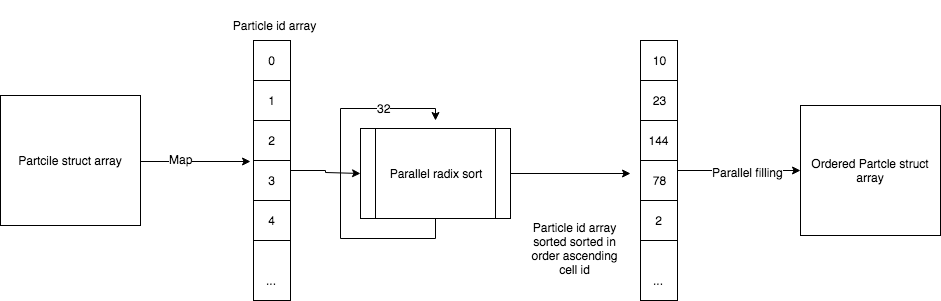
\includegraphics[scale=0.30]{sort1}
  }
  \caption{Схема работы процесса сортировки}\label{fig:sort1}
\end{figure}

\section{Модель вычислений.}\label{sec:ch3/sect3}

Модель вычислений определяет абстрактное представление того, как потоки инструкций выполняются в гетерогенной системе. Управляющая часть программы описывает, структуру, контролирующую ход вычислений и синхронизирует вычислительные узлы. Узел - отдельное независимое устройство GPU/CPU, обладающее изолированной памятью. В зависимости от количества узлов создается соответствующее количество параллельных потоков, выполняющих код обособленно, но в одном адресном пространстве. Каждый поток резервирует узел и контролирует вычисления на нем. Вычисления на узле могут проходить параллельно.

Управляющие конструкции можно разделить на несколько слоев в зависимости от выполняемой задачи. Основной процесс - это абстракция над потоками вычислений, контролирующий процесс инициализации данных и моделей, контроллеров вычислительных утсройств и самих устройств, кроме того, преполагается, что этот процесс отвечает за запуск процесса вычислений и синхронизации данных, а также контроллирует потоки. Колличество решателей соответсвует колличеству физических утсройств, на которых планируется проводить параллелизацию вычислений. Слой решателей состоит из списка экземпляров структур решатель, которая контролирует поток команд для вычилительного устройства, определея тем самым последовотельность запускаемых инструкций, которые, выполняю свою работу обрабатвают тем самым, то подмножетство данных, за которй решатель является ответсвенным. И последний слой - слой устройств на котором опредлеются структуры ответвенные за реализацию паралельных вычислений на конкретном устройстве.
Модель вычислений схематично поилюстрированна на рисунке ~\ref{fig:calc1} ниже.
\begin{figure}[ht]
  \centerfloat{
    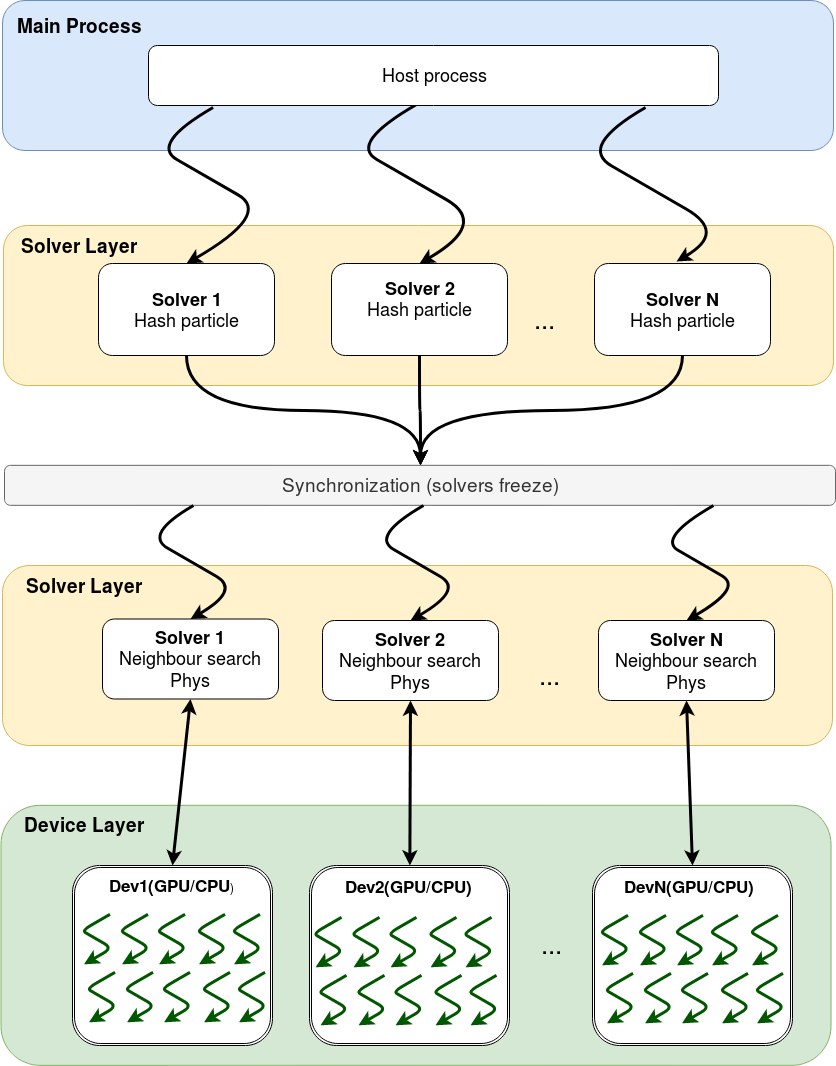
\includegraphics[scale=0.40]{calc1}
  }
  \caption{Модель вычислений.}\label{fig:calc1}
\end{figure}

Как видно из схемы, на этапе синхронизации все потоки  приостанавливаются, и управляющий поток синхронизирует данные между вычислителями, после чего вновь активирует их для дальнейшей работы.

Синхронизация данных включает в себя процесс упорядочивания/сортировки массива частиц по соответствующему значению номера пространственной ячейки, актуализация массивов частиц в оперативной памяти устройств. Как уже было сказано в ~\ref{sec:ch3/sect1} математическая моель среды апроксимируется численной моделью предтавленной в виде множетсва частиц, или массива частиц, если говорить в терминах некоторого языка программирования. Массив представляется как непрерывный участок оперативной паямяти ЭВМ - для того чтобы обеспечить оптимальность выделения памяти каждый эллемент массива выравнивается по полю структы, занимающее наибольший объем пямяти, для структыры частица - это поле velocity, которое занимает 16 байт для архитектуры процессора x86\_64 и при условии использования в качестве базового типа данных чисел одинарной точности. Для синхронизации данных между управляющими потоками и устройствами соответвенно, предлагается использовать стандатные инструменты блокировки, такие как условные переменная и мьютексы \cite{Dijkstra1965}, которые позволяют исключить возможности появления состояний гонки. В момомент синхронизации все контроллеры пытаются захватить мьютекс, тот  которому это удалось сделать, запускает процесс пересчета размера партиций, с учетом, \(\epsilon(d_{i})\) - коэффициента производительности для устройтсва \(d_i\). Затем запускается процесс сортировки массива чатиц. Остальные потоки тем временем ничего не делают и ждут освобождения блокировки, после того как это становится возможным, все данные упорядочены и могут быть загруженны в память устройства. Таким образом устройства могут продолжить свою работу.

\section{Параллельная реализация в системе программирования OpenCL.}\label{sec:ch3/sect4}

Для работы с параллельными вычислениями нами было расмотренно несоклько технологий такие как OpenMP \cite{mattson2019openmp}, CUDA \cite{Cook2012} и OpenCL \cite{Munshi2011, Stone2010}. В силу того что одим из требований к реализации была возможность запуска разрабоатываемой библиотеки на различных видах вычислительных утсройств реализующих технику GPGPU, OpenMP был исключен из этого списка инструметов. В тоже время технология CUDA релизованная и поддерживаемая компанией NVIDIA ограничена в типах устсройств на которых код написанный для компилятора nvcc (NVIDIA CUDA compiller) может быть запущен. Таким образом для работы с параллельными вычислениями была выбрана платформа OpenCL, предназначенная для создания приложений, связанных с вычислениями на гетерогенных вычислительных системах, стандарт обеспечивает параллелизм на уровне инструкций и на уровне данных и является реализацией техники GPGPU  . Основными преимуществами OpenCL являются открытость стандарта и поддержка большинством основных производителей как комплектующих, так и программного обеспечения, например Intel, AMD, NVIDIA, Apple (более подробный список на сайте http://www.khronos.org/opencl/). Таким образом это позволяет писать код, который можно запускать на различных устройствах GPU, CPU, FPGA. Код написанный на языке OpenCL интерпретируется соответствующим  компилятором, например, для GPU от компании NVIDIA компилятор OpenCL встроен в драйвер библиотеки CUDA \cite{Cook2012}. Сравннение технологий приведены ниже в таблице \ref{tab:techCMP}.

\begin{table} [htbp]% Пример записи таблицы с номером, но без отображаемого наименования
  \centering
  \begin{threeparttable}% выравнивание подписи по границам таблицы
    \caption{ Технологии параллельных вычислений. }%
    \label{tab:techCMP}%
    \begin{SingleSpace}
      \begin{tabular}{| c | c | c |}
        \hline
        Название & Открытый (Open source) & Устройства   \\ \hline
        OpenMP   & +                      & CPU          \\ \hline
        CUDA     & -                      & GPU (NVIDIA) \\ \hline
        OpenCL   & +                      & GPU/CPU      \\ \hline
      \end{tabular}%
    \end{SingleSpace}
  \end{threeparttable}
\end{table}

Спецификация OpenCL интерпретирует любую платформу как хост-систему (host) и связанной с одним или более устройством, поддерживающим OpenCL. Каждое устройство состоит из одного или более вычислительных модулей - compute units,  которые  могут  включать  в  себя  несколько обрабатывающих элементов - processing elements. Вычисления  происходят  в обрабатывающих элементах устройства. В данном контексте хост-система выступает в качестве контроллера, управляющего потоком  данных и конвейером вычислений. Обрабатывающие элементы модуля могут выполнять поток инструкций как единицы SIMD(single instruction, multiple data)\cite{Flynn1972} или как единицы SPMD(single program, multiple data streams)\cite{Darema2011}.

Стоит помнить о том, что передача данных по внутренеей шине модуля зачастую быстрее чем обмен данными между хост-программой и модулем. Таким образом данный фактор может стать лимитирующим при неэффективной организации загрузки модуля. Вычисления на устройстве описываются специальными функциями ядрами (kernel) написанными на расширенном диалекте языка С стандарта С99 \cite{Kernighan1988, ISO:C99}. Перед запуском ядра определяется пространство индексов размерность этого пространства в сответствие с стандартом может быть равна 1, 2 или 3. Для каждой точки данного пространства выполняется экземпляр ядра, который называется элементом работы. Соответствующая точка в пространстве индексов задает его глобальный идентификатор. Таким образом при обработки массива данных можно реализовать параллелизм по данным, который является основным сценарием использования OpenCL. Элементы работы объединяются в группы работ, которые обеспечивают более крупнозернистую  декомпозицию пространства индексов. Группам работ также назначаются уникальные идентификаторы, размерность которых совпадает с размерностью пространства индексов. В пределах  одной группы работ каждый элемент получает уникальный локальный идентификатор. Таким образом, элемент работы определяется двумя способами: своим глобальным идентификатором или комбинацией локального идентификатора и идентификатора группы работ ~\ref{fig:ndrange}.
\begin{figure}[ht]
  \centerfloat{
    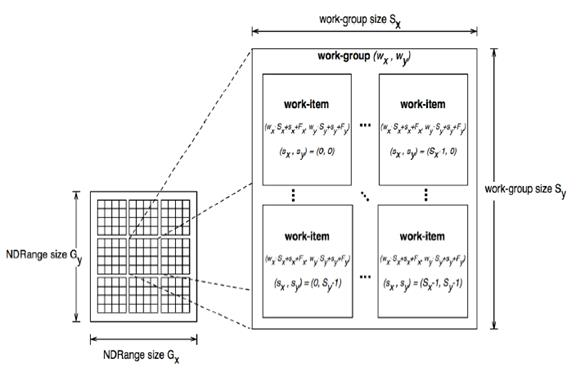
\includegraphics[scale=0.90]{ndrange}
  }
  \caption{Пример индексного пространства NDRange, показывающего рабочие элементы, их глобальные идентификаторы и их сопоставление с парой рабочих групп и локальных идентификаторов.}\label{fig:ndrange}
\end{figure}
Так же OpenCL предатставляет возможность огранизации параллелизма по инструкциям, засчет организации асинхронных конвееров вычислений на основе событийной модели.

Память в стандарте разделяется на несколько категорий в зависимости от типа, размера и скорости доступа:

\begin{itemize}
  \item Глобальная память - оперативная память устройства данная память доступна для чтения и записи всеми элементам работы.
  \item Константная память - выделенная область  глобальной  памяти, которая  доступна только для чтения всем элементам работы и остается постоянной во время исполнения ядра.
  \item Локальная память - пространство памяти доступно для чтенияи записи элементам, принадлежащим одной группе работ, и может эффективно использоваться для доступа к общим переменным. Обычно в качестве такой памяти выступает кеш процессора.
  \item Частная память - несколько регистров памяти, доступной только для чтения и записи лишь одному элементу работы. Переменные, объявленные в частной памяти одного элемента работы, не видимы для другого элемента работы.
\end{itemize}
На рисунке ~\ref{fig:ocl_memory} продемонстрированна расположение раздичных типов памяти для абстрактной вычислительной вычислительной системы с P устройствами.

\begin{figure}[ht]
  \centerfloat{
    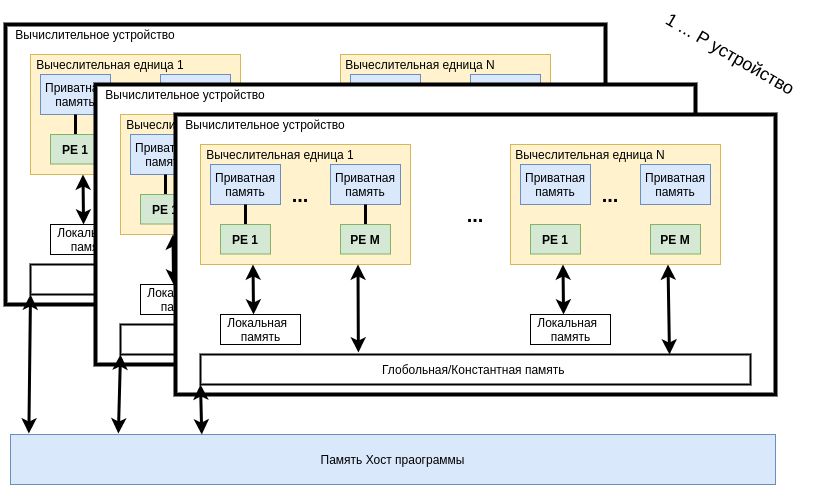
\includegraphics[scale=0.60]{ocl_memory}
  }
  \caption{Типы памяти OpenCL.}\label{fig:ocl_memory}
\end{figure}

Дискретная модель среды или массив частиц помещается в глобальную память устройства. Программа с кодом OpenCL предварительно компилируется соответсвующим компилятором, предоставляемым вместе с библиотекой для кокретного устройтсва. Кроме компилятора библиотека содержит в себе среду выполнения, которая контроллирует ход вычислений, следит за очередью задач, и драйвер устройтсва. При компиляции ядра код проходин несколько стадий \cite{Hong2014} на каждом этапе происходит преобразование кода.

На первом этапе исходный код на OpenCL C транслируется в промежуточное представление на языке LLVM IR \cite{Lattner2004, Lattner2002}. LLVM (Low Level Virtual Machine) — является средой для создание компиляторов и утилит, на данный момент реализованно весьма широкий спектр компиляторов для различных языков программирования в том числе для C, C++, Java, OpenCL C, CUDA и так даллее. В основе LLVM используется платформонезависимая система кодирования машинных инструкций LLVM IR, которая позволяет интерпретировать код программы в платформно независмимуб форму - так называемый байткод после чего компилятор может пременять ряд преобразований и трансформаций для оптимизации такие как анализ графа вызовов и сопостовление образцов, помогающее выявлять ожидаемое поведние в части кода, соответвующиму определенному паттерну. И, наконец, на финальной стадии отимизированный код на языке LLVM IR компилируется в машинный код для заданной платформы и операционной системы.
На рисунке ~\ref{fig:ocl_compiller} проилюстрированны этапы компиляции оптимизации и построения кода для рабочей среды OpenCL устройства.

\begin{figure}[ht]
  \centerfloat{
    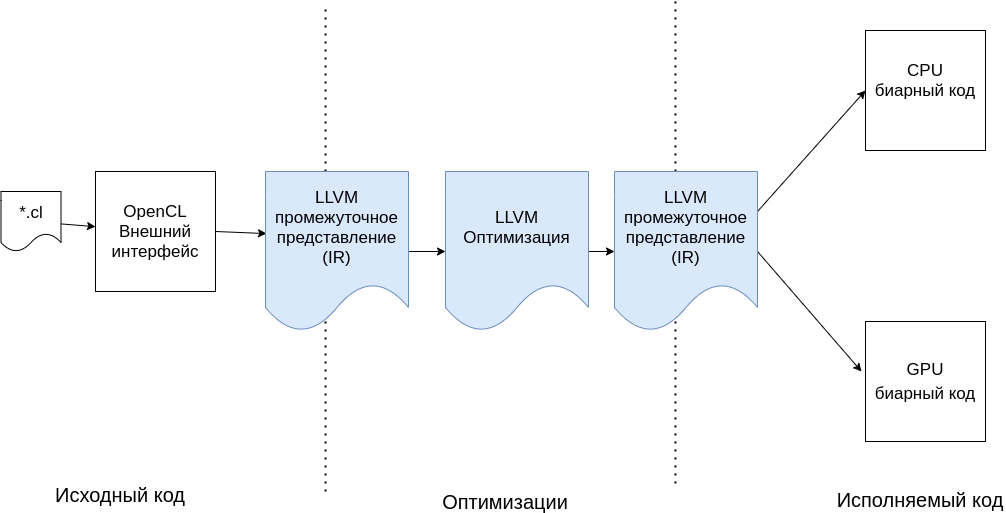
\includegraphics[scale=0.45]{ocl_compilation_stages}
  }
  \caption{Этапы компиляции программы для OpenCL платформ.}\label{fig:ocl_compiller}
\end{figure}

Таким образом подобное преобразование помогает абстрагировать OpenCL код от конретной платформы и устройства (CPU, GPU, FPGA) и делает его более гибким и переносимым. На данный момент весь код, содержащий инструкции для среды выполнения кода OpenCL содержатся в 11 функциях ядрах:
\begin{itemize}
  \item kernel\_init\_ext\_particles  - инициализация списков соседей.
  \item kernel\_hash\_particles - расчет пространственного хеша.
  \item kernel\_clear\_grid\_hash, kernel\_fill\_particle\_cell\_hash - процедуры предварительной подготовки дополнительных струкутр данных необходимых для поиска соседей.
  \item kernel\_neighbour\_search - процедура поиска соседей для каждой частицы
  \item kernel\_compute\_forces\_init\_pressure - инициализация векторов внешних сил \(F^{external}\) и давдения \(F^{pressure}\) нулем.
  \item kernel\_predict\_positions - вычисление текущего расположения частиц с учетом текущих значений физических параметров.
  \item kernel\_predict\_density - вычисление текущего значения плотности в зависимости от расположения частиц
  \item kernel\_correct\_pressure - корректеровка давления.
  \item kernel\_compute\_pressure\_force\_acceleration - прерасчет позиций частиц в соответсивие со скорентированным давлением.
  \item kernel\_integrate - этап интеграции, расчет конечного положения частиц и их скоростей.
\end{itemize}

Стоит отметить, что расчеты происходят параллельно и независимо для каждой частицы, которая попадает в подмножество обрабатывамое конкретным устройством.
Для паралельной сортировки OpenCL код состоит из шести ядер:
\begin{itemize}
  \item kernel\_prepare - подготовка структур.
  \item kernel\_count - постороение локального распределения.
  \item kernel\_scan - ... \fixme{дописать}
  \item kernel\_coalesce - ... \fixme{дописать}
  \item kernel\_reorder - перестроенние списка индексов.
  \item kernel\_shuffle - перераспределение множества частиц.
\end{itemize}
